% sys-optimization.tex — \input'd from experiments/experiments.tex
%
% Sensitivity analysis and gradient-based improvement of the systolic ratio.
%
% Sources:
%   - Generated data: experiments/sys-optimization/sys-optimization-sensitivity.jsonl
%   - Generated data: experiments/sys-optimization/sys-optimization-steps.jsonl
%   - Plot script: experiments/sys-optimization/sys_optimization.py
%   - Experiment notes: experiments/sys-optimization/README.md
%
% Structure:
%   - Motivation and approach
%   - Derivative computation (formal lemmas)
%   - Step bound algorithm
%   - Sensitivity analysis (Phase 1)
%   - Finite gradient steps (Phase 2)
%   - Discussion

\subsection{Sensitivity Analysis and Gradient Optimization of sys}
\label{sec:sys-optimization}

Random sampling has not found $\mathrm{sys} > 1$ (see
Sections~\ref{sec:random-sweep} and~\ref{sec:random-product-sweep}).
Instead of relying on random exploration, we compute the gradient
$\nabla_h\,\mathrm{sys}$ of the systolic ratio with respect to the
facet heights $h = (h_1,\dots,h_F)$ and take directed steps to increase
$\mathrm{sys}$.

\subsubsection*{Method}

For a polytope $K = \{x \in \mathbb{R}^4 \mid n_k \cdot x \le h_k,\; k=1,\dots,F\}$
with unit outward normals $n_k$, the systolic ratio decomposes as
$\mathrm{sys} = c_{\mathrm{EHZ}}^2 / (2\,\mathrm{vol})$.
We compute the sensitivity of each factor to individual height changes.

All quantities needed for the gradient ($\beta^*$, $\nu$, $Q^*$, facet
volumes $S_k$) are either already computed by the HK2017 algorithm's
KKT solve or can be extracted from the polytope data at negligible
additional cost. A single pass of HK2017 thus provides the full
sensitivity analysis.

We first state the general principle, then apply it to our setting.

\begin{theorem*}[Envelope theorem for constrained optimization]
Let $f(x;\theta)$ be a smooth objective and $g_i(x;\theta) = 0$,
$i = 1,\dots,m$, smooth equality constraints, with parameter $\theta$.
Let $x^*(\theta)$ be a non-degenerate KKT point with multipliers
$\lambda^*(\theta)$, and let
$\mathcal{L}(x,\lambda;\theta) = f(x;\theta) - \sum_i \lambda_i g_i(x;\theta)$
be the Lagrangian.
Then the optimal value $f^*(\theta) = f(x^*(\theta);\theta)$ satisfies
\[
  \frac{\partial f^*}{\partial \theta}
  = \frac{\partial \mathcal{L}}{\partial \theta}\bigg|_{x=x^*,\,\lambda=\lambda^*}
  = \frac{\partial f}{\partial \theta}\bigg|_{x^*}
    - \sum_i \lambda_i^* \frac{\partial g_i}{\partial \theta}\bigg|_{x^*}.
\]
\end{theorem*}

\begin{lemma}[Volume derivative]
\label{lem:vol-derivative}
For a convex polytope $K$ in $H$-representation with unit normals,
\[
  \frac{\partial\,\mathrm{vol}(K)}{\partial h_k} = S_k,
\]
where $S_k = \mathrm{vol}_{3}(F_k)$ is the $3$-dimensional volume of facet $F_k$.
\end{lemma}

\begin{proof}
Moving facet $k$ outward by $\delta$ enlarges $K$ to
$K' = K \cup \{x : h_k < n_k \cdot x \le h_k + \delta,\; n_j \cdot x \le h_j \;\forall j \ne k\}$.
The cross-section at $n_k \cdot x = h_k + t$ equals the facet $F_k$ at $t = 0$
and varies continuously.
Thus $\mathrm{vol}(K') - \mathrm{vol}(K) = \delta \cdot S_k + O(\delta^2)$.
\end{proof}

Facet volumes are computed via ridge-based tetrahedralization:
for each facet, pick the centroid of its vertices as apex, fan-triangulate
each ridge (a 2-face shared with another facet), and sum the 3D tetrahedron
volumes via the 4D cross product.
This is cross-checked against the divergence theorem
$\mathrm{vol}(K) = \frac{1}{4}\sum_k h_k\,S_k$ (agreement to $< 5 \times 10^{-8}$ relative error)
and against central finite differences with step size $10^{-3}$
(agreement to $< 5\%$; smaller step sizes suffer from qhull volume noise).

\begin{lemma}[Capacity derivative via envelope theorem]
\label{lem:cap-derivative}
Fix an orbit $(S,\sigma)$ with $|S| = m$ facets. The orbit's action is
$A(S,\sigma;h) = 1/(2\,Q^*)$, where $Q^*$ is the maximum of the KKT problem
\[
  Q(\beta) = \tfrac{1}{2}\beta^T H \beta
  \quad\text{subject to}\quad
  N^T\beta = 0,\; \eta^T\beta = 1,
\]
with $\eta_i = h_{\sigma(i)}$, $i = 1,\dots,m$.
Let $\nu$ be the Lagrange multiplier for the normalization constraint
$\eta^T\beta = 1$ at the optimum.
If facet $k$ appears in the orbit at position $i_0$ (i.e.\ $\sigma(i_0) = k$), then
\[
  \frac{\partial A}{\partial h_k}
  = \frac{\nu\,\beta_{i_0}^*}{2\,(Q^*)^2}.
\]
If $k \notin S$, then $\partial A / \partial h_k = 0$.
\end{lemma}

\begin{proof}
The Lagrangian is
$\mathcal{L}(\beta,\lambda,\nu) = \tfrac{1}{2}\beta^T H\beta - \lambda^T N^T\beta - \nu(\eta^T\beta - 1)$.
The heights enter only through $\eta$, and $\partial\eta_i/\partial h_k = \delta_{\sigma(i),k}$.
By the envelope theorem,
$\partial Q^*/\partial h_k = \partial\mathcal{L}/\partial h_k = -\nu\,\beta_{i_0}^*$.
Since $A = 1/(2Q)$, the chain rule gives
$\partial A/\partial h_k = -(\partial Q^*/\partial h_k) / (2\,(Q^*)^2) = \nu\,\beta_{i_0}^* / (2\,(Q^*)^2)$.
\end{proof}

\begin{proposition}[Capacity as piecewise-smooth function of heights]
\label{prop:capacity-piecewise-smooth}
Let $K(h)$ be a polytope with fixed normals and variable heights~$h$.
\begin{enumerate}
\item[\textup{(a)}]
  \emph{Combinatorial type stability.}
  For each $h_0$ such that $K(h_0)$ is a polytope, the vertex-facet
  incidence graph is locally constant: there exists $\varepsilon > 0$ such that
  $K(h)$ has the same combinatorial type for all $\|h - h_0\| < \varepsilon$.
  In particular, the set of valid orbit nodes $(S,\sigma)$ surviving
  the HK2017 pruning is constant in this neighborhood.

\item[\textup{(b)}]
  \emph{Per-orbit smoothness.}
  Fix an orbit $(S,\sigma)$ whose KKT problem has a unique non-degenerate
  maximum. Then the action $A(S,\sigma;\cdot)$ is smooth in~$h$,
  with derivative given by Lemma~\ref{lem:cap-derivative}.

\item[\textup{(c)}]
  \emph{Capacity at generic heights.}
  The capacity $c_{\mathrm{EHZ}}(h) = \min_{(S,\sigma)} A(S,\sigma;h)$
  is continuous.
  At heights where the minimizing orbit is unique, $c_{\mathrm{EHZ}}$ is
  differentiable with gradient given by that orbit's envelope theorem
  formula. This is the generic case: having two orbits with equal action
  is a codimension-$1$ condition in height space.

\item[\textup{(d)}]
  \emph{Capacity at orbit-switching boundaries.}
  When $r \ge 2$ orbits $(S_1,\sigma_1),\dots,(S_r,\sigma_r)$ achieve
  the minimum action simultaneously, the capacity is non-smooth.
  The directional derivative in direction~$d$ is
  \[
    D_d\,c_{\mathrm{EHZ}}(h)
    = \min_{i=1,\dots,r} \nabla_h A(S_i,\sigma_i;h) \cdot d,
  \]
  i.e.\ the most pessimistic rate of change among the tied orbits.
  Stepping in a direction where a \emph{different} orbit gives the
  minimum rate can cause the actual capacity to deviate from the
  prediction based on the current minimizer (\emph{orbit switching}).
\end{enumerate}
\end{proposition}

\begin{proof}[Proof sketch]
(a) The vertices of $K(h)$ depend continuously on~$h$ (they are solutions
of $4 \times 4$ linear systems in the normals and heights). Vertex-on-facet
incidence $n_j \cdot v = h_j$ is an open condition to violate, so it
persists under small perturbations.
(b) Follows from the envelope theorem applied to the KKT problem, whose
optimum is locally unique and smooth by the implicit function theorem.
(c) Continuity: $\min$ of continuous functions.
Differentiability: when the minimizer is unique, $c_{\mathrm{EHZ}} =
A(S^*,\sigma^*;\cdot)$ locally, hence smooth by~(b).
The codimension-$1$ claim follows because $A(S_1,\sigma_1;h) = A(S_2,\sigma_2;h)$
is generically a single equation in $F$ unknowns.
(d) Standard result for the directional derivative of a pointwise minimum
of smooth functions.
\end{proof}

\emph{Validity of the single-orbit gradient.}
In our experiment, we compute $\nabla_h\,c_{\mathrm{EHZ}}$ using only
the current minimizing orbit. By Proposition~\ref{prop:capacity-piecewise-smooth}(c),
this is exact whenever the minimizer is unique.
When the runner-up gap $\Delta = A_{\mathrm{runner\text{-}up}} - A_{\mathrm{best}}$
is positive, the gradient remains valid for step sizes~$t$ small enough
that no orbit switch occurs, roughly $t \lesssim \Delta / |\text{rate difference}|$.
In our dataset, 73 of 132 multi-orbit polytopes (55\%) have a relative gap
$\Delta/A > 10^{-3}$, and 126 of 140 polytopes improve after a finite step,
suggesting that the single-orbit gradient is a reliable heuristic for
moderate step sizes.
Among the 14 polytopes that do not improve, most either sit at an
orbit-switching boundary ($\Delta \approx 0$) or have improvements
below numerical noise ($|\Delta\,\mathrm{sys}| < 10^{-9}$).

\emph{Systolic ratio derivative.}
The chain rule gives
\[
  \frac{\partial\,\mathrm{sys}}{\partial h_k}
  = \frac{1}{\mathrm{vol}}
    \left[
      c_{\mathrm{EHZ}} \cdot \frac{\partial\,c_{\mathrm{EHZ}}}{\partial h_k}
      - \mathrm{sys} \cdot \frac{\partial\,\mathrm{vol}}{\partial h_k}
    \right].
\]

\emph{Step bound.}
We step along $g = \nabla_h\,\mathrm{sys}$, setting $h' = h + t\,g$.
To preserve the combinatorial type, we require:
(i)~all heights remain positive ($h_k + t\,g_k > 0$), and
(ii)~no vertex crosses a new facet.
For a simple vertex $v$ (exactly 4 determining facets with normals
forming an invertible matrix $N_v$), the vertex moves as
$v(t) = v + t\,N_v^{-1}g_{\mathrm{det}}$.
For each non-incident facet $j$, the slack $s_j(t) = h_j + t\,g_j - n_j \cdot v(t)$
must remain positive; this gives $t < s_j(0)/(-\dot{s}_j)$ when the slack is
decreasing.
For non-simple vertices (more than 4 incident facets, common in
Lagrangian products), a conservative bound $t < s_j / \max_k |g_k|$ is used.
The step bound is $t_{\max} = \min$ over all such critical times, capped at~$100$.

We evaluate $\mathrm{sys}$ at step fractions
$\{0.1, 0.25, 0.5, 0.75, 0.95\} \cdot t_{\max}$.

The starting polytopes are the 140 polytopes from the random-sweep and
random-product-sweep experiments with $F \le 10$.

\subsubsection*{Phase 1: Gradient Structure}

Figure~\ref{fig:sys-opt-gradient} shows the distribution of gradient
magnitudes $|{\partial\,\mathrm{sys}}/{\partial h_k}|$ across all
polytopes and facets.

\begin{figure}[h]
\centering
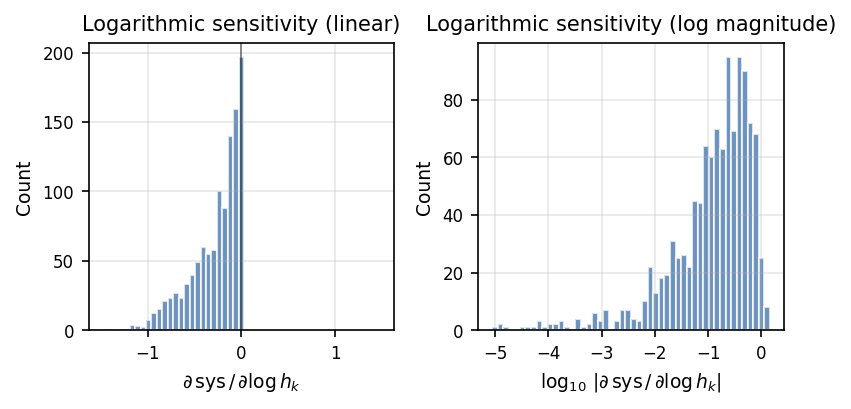
\includegraphics[width=\textwidth]{../experiments/sys-optimization/sys_optimization_gradient_hist.png}
\caption{Distribution of gradient magnitudes $|{\partial\,\mathrm{sys}}/{\partial h_k}|$
  across 1120 facets from 140 polytopes.
  Left: linear scale. Right: log scale.}
\label{fig:sys-opt-gradient}
\end{figure}

\begin{figure}[h]
\centering
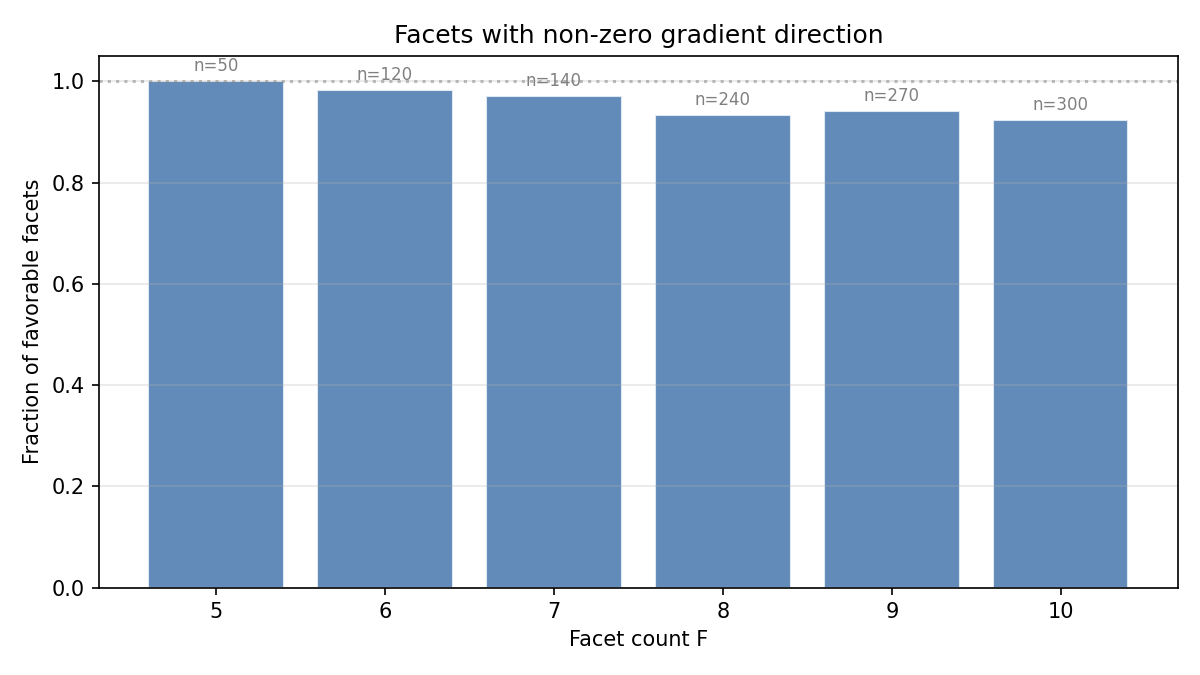
\includegraphics[width=0.75\textwidth]{../experiments/sys-optimization/sys_optimization_favorable.png}
\caption{Fraction of facets per polytope with $|{\partial\,\mathrm{sys}}/{\partial h_k}| > 0$,
  grouped by facet count.}
\label{fig:sys-opt-favorable}
\end{figure}

Every polytope in our dataset has a non-zero gradient:
$\|\nabla_h\,\mathrm{sys}\| > 0$ for all 140 polytopes.
Over 96\% of individual facets provide a direction that changes
$\mathrm{sys}$, meaning that almost every facet height can be adjusted
to either increase or decrease the systolic ratio.

\subsubsection*{Phase 2: Finite Gradient Steps}

Figure~\ref{fig:sys-opt-improvement} shows the result of taking the best
single gradient step for each polytope.

\begin{figure}[h]
\centering
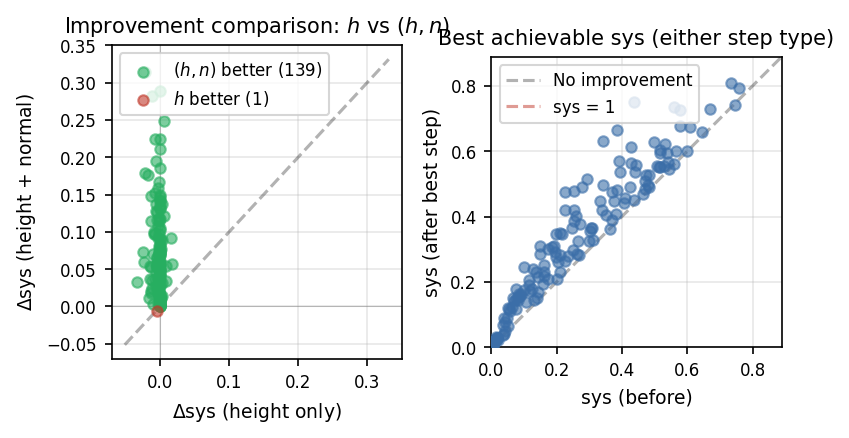
\includegraphics[width=0.65\textwidth]{../experiments/sys-optimization/sys_optimization_improvement.png}
\caption{Systolic ratio before vs.\ after the best gradient step.
  Points above the diagonal represent improvement.
  The dashed lines mark $\mathrm{sys} = 1$.}
\label{fig:sys-opt-improvement}
\end{figure}

\begin{table}[h]
\centering
\begin{tabular}{lr}
\toprule
Statistic & Value \\
\midrule
Polytopes analyzed & 140 \\
Polytopes with $\|\nabla \mathrm{sys}\| > 0$ & 140 \\
Polytopes improved by gradient step & 126 \\
Best sys (before) & 0.7579 \\
Best sys (after step) & 0.8049 \\
Mean $\Delta$sys (best step) & 0.0341 \\
Median $\Delta$sys (best step) & 0.0138 \\
Mean $\|\nabla \mathrm{sys}\|$ & 0.1923 \\
\bottomrule
\end{tabular}

\caption{Summary statistics for the sys-optimization experiment.}
\label{tab:sys-opt-stats}
\end{table}

Of the 140 starting polytopes, 126 (90\%) show an improved $\mathrm{sys}$
after a single gradient step.
The mean improvement is $\Delta\,\mathrm{sys} = 0.034$ and the median is~$0.014$.
The best $\mathrm{sys}$ achieved is~$0.805$, starting from a polytope
with $\mathrm{sys} = 0.758$ (a random $4 \times 5$ Lagrangian product).

\subsubsection*{Discussion}

No single gradient step pushes $\mathrm{sys}$ past~$1$.
The best result ($\mathrm{sys} \approx 0.80$) remains well below the
Viterbo threshold, though it exceeds the maximum
$\mathrm{sys} \approx 0.76$ found by random sampling alone.

Two structural observations:
\begin{enumerate}
\item \emph{The gradient is never zero.}
  None of the 140 polytopes is a local optimum of $\mathrm{sys}$ under
  height changes. Every polytope admits a direction of improvement.
  This suggests that $\mathrm{sys}$ does not have local maxima in
  height space (at least not in the explored region), consistent with a
  picture where $\mathrm{sys}$ increases monotonically toward a
  global optimum or toward a boundary of the feasible region.

\item \emph{Orbit switching limits finite steps.}
  As shown in Proposition~\ref{prop:capacity-piecewise-smooth}(d),
  a different orbit may become the minimizer after a finite step,
  causing the actual $\mathrm{sys}$ change to differ from the
  gradient's prediction.
  For higher facet counts ($F \ge 8$), the step bound
  $t_{\max}$ before a combinatorial type change is typically small
  ($t_{\max} < 1$), further limiting per-step improvement.
  Iterating the gradient step across combinatorial type changes
  (Phase~3) would require re-instrumenting HK2017 after each type
  change.
\end{enumerate}

These results motivate Phase~3 (iterative optimization) and Phase~1c
(adding facets), which could potentially reach higher $\mathrm{sys}$
values by exploring beyond single gradient steps.
